\documentclass[10pt,letterpaper]{article}
\usepackage[top=0.85in,left=2.75in,footskip=0.75in]{geometry}

% amsmath and amssymb packages, useful for mathematical formulas and symbols
\usepackage{amsmath,amssymb}

% Use adjustwidth environment to exceed column width (see example table in text)
\usepackage{changepage}

% textcomp package and marvosym package for additional characters
\usepackage{textcomp,marvosym}

% cite package, to clean up citations in the main text. Do not remove.
\usepackage{cite}

% Use nameref to cite supporting information files (see Supporting Information section for more info)
\usepackage{nameref,hyperref}

% line numbers
\usepackage[right]{lineno}

% ligatures disabled
\usepackage[nopatch=eqnum]{microtype}
\DisableLigatures[f]{encoding = *, family = * }

% color can be used to apply background shading to table cells only
%\usepackage[table]{xcolor}

% array package and thick rules for tables
\usepackage{array}

% create "+" rule type for thick vertical lines
\newcolumntype{+}{!{\vrule width 2pt}}

% create \thickcline for thick horizontal lines of variable length
\newlength\savedwidth
\newcommand\thickcline[1]{%
  \noalign{\global\savedwidth\arrayrulewidth\global\arrayrulewidth 2pt}%
  \cline{#1}%
  \noalign{\vskip\arrayrulewidth}%
  \noalign{\global\arrayrulewidth\savedwidth}%
}

% \thickhline command for thick horizontal lines that span the table
\newcommand\thickhline{\noalign{\global\savedwidth\arrayrulewidth\global\arrayrulewidth 2pt}%
\hline
\noalign{\global\arrayrulewidth\savedwidth}}


% Remove comment for double spacing
%\usepackage{setspace} 
%\doublespacing

% Text layout
\raggedright
\setlength{\parindent}{0.5cm}
\textwidth 5.25in 
\textheight 8.75in

% Bold the 'Fig #' in the caption and separate it from the title/caption with a period
% Captions will be left justified
\usepackage[aboveskip=1pt,labelfont=bf,labelsep=period,justification=raggedright,singlelinecheck=off]{caption}
\renewcommand{\figurename}{Fig}

% Use the PLoS provided BiBTeX style
\bibliographystyle{plos2015}

% Remove brackets from numbering in List of References
\makeatletter
\renewcommand{\@biblabel}[1]{\quad#1.}
\makeatother


% Header and Footer with logo
\usepackage{lastpage,fancyhdr,graphicx}
\usepackage{epstopdf}
\usepackage{lmodern}
%\pagestyle{myheadings}
\pagestyle{fancy}
\fancyhf{}
%\setlength{\headheight}{27.023pt}
%\lhead{\includegraphics[width=2.0in]{PLOS-submission.eps}}
\rfoot{\thepage/\pageref{LastPage}}
\renewcommand{\headrulewidth}{0pt}
\renewcommand{\footrule}{\hrule height 2pt \vspace{2mm}}
\fancyheadoffset[L]{2.25in}
\fancyfootoffset[L]{2.25in}
\lfoot{\today}

%% Include all macros below

\newcommand{\lorem}{{\bf LOREM}}
\newcommand{\ipsum}{{\bf IPSUM}}

%% END MACROS SECTION

%% personal packages and macro
%%% packages
\usepackage[utf8]{inputenc}        % allow utf-8 input
\usepackage[T1]{fontenc}           % use 8-bit T1 fonts
\usepackage[dvipsnames, table]{xcolor}
\usepackage{tabularx}
\usepackage{multirow}
\usepackage{pifont}
\usepackage{csvsimple}
\usepackage[font={small},textfont={it},labelfont={bf}]{caption}
\usepackage{subcaption}
\usepackage{graphicx}
\usepackage{url}                   % simple URL typesetting
\usepackage{booktabs}              % professional-quality tables
\usepackage{makecell}
\usepackage{amsfonts}              % blackboard math symbols
\usepackage{amsmath}
\usepackage{nicefrac}              % compact symbols for 1/2, etc.
\usepackage{microtype}             % microtypography
\usepackage{enumitem}
\usepackage[export]{adjustbox}


%not compatible with cite package
%\usepackage[natbib=true,style=nature,maxnames=999,maxcitenames=2,backend=biber]{biblatex}
%\addbibresource{references.bib}

%%% macros
\DeclareMathOperator*{\argmin}{arg\,min}
\newcommand{\indep}{\perp \!\!\! \perp}
\newtheorem{assumption}{Assumption}

\definecolor{dark_blue}{rgb}{0,0,.65}
\definecolor{dark_green}{rgb}{0,.5,.15}

\hypersetup{pdftex,  % needed for pdflatex
  breaklinks=true,  % so long urls are correctly broken across lines
  colorlinks=true,
  linkcolor=dark_blue,
  citecolor=dark_green,
}
\colorlet{P}{ForestGreen}
\colorlet{I}{MidnightBlue}
\colorlet{C}{YellowOrange}
\colorlet{O}{DarkOrchid}
\colorlet{T}{Gray}

\begin{document}
\vspace*{0.2in}

% Title must be 250 characters or less.
\begin{flushleft}
  {\Large
    \textbf\newline{Step-by-step causal analysis of EHRs to ground decision-making} % Please use "sentence case" for title and headings (capitalize only the first word in a title (or heading), the first word in a subtitle (or subheading), and any proper nouns).
  }
  \newline
  % Insert author names, affiliations and corresponding author email (do not include titles, positions, or degrees).
  \\
  Matthieu Doutreligne\textsuperscript{1,2,*},
  Tristan Struja\textsuperscript{3,4},
  Judith Abecassis\textsuperscript{1},
  Claire Morgand\textsuperscript{5},
  Leo Anthony Celi\textsuperscript{3,6,7},
  Gaël Varoquaux\textsuperscript{1}
  \bigskip
  \\
  \textbf{1} Soda Team, Inria Saclay, Palaiseau, France
  \\
  \textbf{2} Mission Data, Haute Autorité de Santé, Saint-Denis, France
  \\
  \textbf{3} Laboratory for Computational Physiology, Massachusetts Institute of Technology, Cambridge, Massachusetts, United States of America
  \\
  \textbf{4} Medical University Clinic, Division of Endocrinology, Diabetes \& Metabolism, Kantonsspital Aarau, Aarau, Switzerland
  \\
  \textbf{5} Agence Régionale de Santé Ile-de-France, Saint-Denis, France
  \\
  \textbf{6} Division of Pulmonary, Critical Care and Sleep Medicine, Beth Israel Deaconess Medical Center, Boston, Massachusetts, United States of America
  \\
  \textbf{7} Department of Biostatistics, Harvard T.H. Chan School of Public Health, Boston, Massachusetts, United States of America
  \bigskip




  % Insert additional author notes using the symbols described below. Insert symbol callouts after author names as necessary.
  % 
  % Remove or comment out the author notes below if they aren't used.
  %
  % Primary Equal Contribution Note
  %\Yinyang Corresponding author: m.doutreligne@has-sante.fr.

  % Additional Equal Contribution Note
  % Also use this double-dagger symbol for special authorship notes, such as senior authorship.
  %\ddag These authors also contributed equally to this work.

  % Current address notes
  %\textcurrency Current Address: Dept/Program/Center, Institution Name, City, State, Country % change symbol to "\textcurrency a" if more than one current address note
  % \textcurrency b Insert second current address 
  % \textcurrency c Insert third current address

  % Deceased author note
  %\dag Deceased

  % Group/Consortium Author Note
  %\textpilcrow Membership list can be found in the Acknowledgments section.

  % Use the asterisk to denote corresponding authorship and provide email address in note below.
  * Corresponding author: m.doutreligne@has-sante.fr


\end{flushleft}
% Please keep the abstract below 300 words --> 235
\section*{Abstract}

Causal inference enables machine learning methods to estimate treatment effects
of medical interventions from electronic health records (EHRs). The prevalence
of such observational data and the difficulty for randomized controlled trials (RCT) to cover all
population/treatment relationships make these methods increasingly attractive
for studying causal effects. However, researchers should be wary of many
pitfalls.

We propose and illustrate a framework for causal inference estimating the
effect of albumin on mortality in sepsis using an Intensive Care database
(MIMIC-IV) and comparing various sensitivity analyses to results from RCTs as gold-standard.

The first step is study design, using the target trial concept and the PICOT
framework: Population (patients with sepsis), Intervention (combination of
crystalloids and albumin for fluid resuscitation), Control (crystalloids only),
Outcome (28-day mortality), Time (intervention start within 24h of admission).
We show that too large treatment-initiation times induce immortal time bias.
The second step is selection of the confounding variables based on expert
knowledge. Increasingly adding confounders enables to recover the RCT results
from observational data. As the third step, we assess the influence
of multiple models with varying assumptions, showing that a doubly robust estimator (AIPW)
with random forests proved to be the most reliable estimator. Results show that
these steps are all important for valid causal estimates. A valid causal model
can then be used to individualize decision making: subgroup analyses showed that
treatment efficacy of albumin was better for patients >60 years old, males, and
patients with septic shock.

Without causal thinking, machine learning is not enough for optimal clinical
decision on an individual patient level. Our step-by-step analytic framework helps avoiding many pitfalls of applying machine learning to EHR data,
building models that avoid shortcuts and extract the best decision-making evidence.

% Please keep the Author Summary between 150 and 200 words
% Use first person. PLOS ONE authors please skip this step. 
% Author Summary not valid for PLOS ONE submissions.   
\section*{Author summary}

Rich routine-care data, as EHR or claims, is useful to individualize decision
making using machine learning; but guiding interventions requires
causal inference. Unlike with an RCT, interventions in routine data do
not easily enable an apple-to-apple measure of the effect of an
intervention, leading to many analytical pitfalls, particularly in
time-varying data. We study these in a tutorial spirit, making
the code and data openly available. We give 5 analytical steps for
data-driven individualized interventions: Step
1) Study design, where common pitfalls are selection bias, with information
unequally collected across treatment and control patients, and immortal time
bias, where the inclusion-defining event interacts with the
intervention time. Step 2) Identification of the causal assumptions and
categorization of confounders. Step 3) Estimation of the causal effect of
interest by correct aggregation of confounders and selection of an appropriate
statistical model. Step 4) Assessing the
analysis' robustness to assumptions, and finally Step 5) Individualizing
treatment decision, by exploring treatment heterogeneity, eg across subgroups.
Studying choice of fluid resuscitation in sepsis, we show that common
mistakes in steps 1, 2, and 3 equally compromise causal validity.


\linenumbers

% Use "Eq" instead of "Equation" for equation citations.
\section*{Introduction: data-driven decisions require causal inference}
%\label{introduction}

Informing a care option extends beyond merely predicting the occurrence
of an event; it involves estimating the effect of the corresponding
treatment effects. Routine-care data comes naturally to mind to guide
routine decisions, but they require care to estimate treatment effects as
they are observational, unlike Randomized controlled trials (RCTs). This
context calls for causal inference statistical frameworks.
But merely applying these tools to the data does suffice to ensure the
validity of the inferences; numerous considerations must be carefully addressed.

\paragraph{Individualized Medicine and Machine Learning Challenges}
Machine learning plays a pivotal role in individualized medicine  \cite{rajkomar2018scalable,liu2019comparison,li2020behrt,beaulieu2021machine,aggarwal2021diagnostic}. It
demonstrated superior performance over traditional rule-based clinical scores in predicting a patient's readmission risk, mortality, or future comorbidities using Electronic Health Records (EHRs) \cite{rajkomar2018scalable,liu2019comparison,li2020behrt,beaulieu2021machine,aggarwal2021diagnostic}.
However, mounting evidence suggests that machine-learning models can inadvertently perpetuate and exacerbate biases present in the data \cite{rajkomar2018ensuring}, including gender or racial biases \cite{singh2022generalizability,gichoya2022ai}, and the marginalization of under-served populations \cite{seyyed2021underdiagnosis}. These biases are typically encoded by capturing shortcuts—stereotypical or distorted features in the data \cite{geirhos2020shortcut,winkler2019association,degrave2021ai}.
%
For instance, numerous machine learning algorithms rely on post-treatment information \cite{badgeley2019deep,obermeyer2019dissecting,yuan2021temporal,wong2021external}, exemplified by a diagnostic model for skin cancer that depends on surgical marks \cite{winkler2019association}. For Intensive Care Unit data, focus of our study, such information markedly improves mortality prediction (S1 Fig), but cannot inform decisions.

\paragraph{The Importance of Causal Reasoning in Data-Driven Decision-Making} \cite{prosperi2020causal}
While conventional machine learning relies on retrospective to generate predictions of future effects \cite{plecko2022causal}, truly informing decision-making needs a comparison of potential outcomes with and without the intervention. This involves estimating a causal effect, mirroring the methodology employed in RCTs \cite{prosperi2020causal}. However, RCTs encounter challenges such as selection biases \cite{travers2007external,averitt2020translating}, difficulties in recruiting diverse populations, and limited sample sizes for exploring treatment heterogeneity across subgroups. Routinely collected data presents a unique opportunity to assess real-life benefit-risk trade-offs associated with a decision \cite{desai2021broadening}, with reduced sampling bias and sufficient data to capture heterogeneity \cite{rekkas2023standardized}. Nevertheless, estimating causal effects from such data is challenging due to the confounding of the intervention by indication. Therefore, dedicated statistical techniques are imperative to emulate a "target trial" \cite{hernan2016specifying} from observational data.

% \paragraph{How lack of individual treatment model limits a cardiovascular risk
% score} The QRISK is a risk score widely used in the UK to assess 10-year and
% lifetime cardio-vascular risk \cite{hippisley2017development}. It is well
% calibrated, recommended by the national regulatory agency
% \cite{guideline2023cardiovascular}, and the National Institute for Health and
% Care Excellence (NICE) argues to use such a score to systematically screen
% cardio-vascular disease (CVD) risks and treat with statins individuals at risk
% \cite{guideline2023cardiovascular}, especially if 10-year CVD risk exceeds
% 10\% \cite{rabar2014lipid}.  A cost-effectiveness analysis guided the choice
% of the 10\% threshold to optimize quality-adjusted life years at the
% population level \cite{guthrie2023competing}. The NICE analysis is based on
% evidence mostly from three trials, accounting for more than 70\% of the
% effect: LIPID \cite{long1998prevention} (32\% of the effect), PROSPER
% \cite{shepherd2002pravastatin} (22\% of the effect), ALLHAT-LLT
% \cite{antihypertensive2002major} (23\% of the effect). All these trials
% focused on high-risk patients and secondary prevention. All studies operate
% under the assumption of a consistent statin effect (risk ratios constant)
% across different CVD risk groups, irrespective of the baseline CVD risk and
% LDL-cholesterol levels. This aligns with the outcomes of two meta-analyses
% which observed broadly similar effectiveness across risk levels
% \cite{brugts2009benefits}, but is challenged by another study in primary
% prevention \cite{byrne2019statins}. Meanwhile the US Preventive Services Task
% Force concluded that the evidence is insufficient to determine the balance of
% benefits and harms of statin use for the primary prevention of CVD events and
% mortality in adults 76 years and older \cite{chou2022statin}.

% \paragraph{Critics on the efficiency of systematic screening and treatment heterogeneity}
% Conversely, the World Health Organization (WHO) published a systematic review on
% screening for CVD risk in 2019 \cite{eriksen2021effectiveness} asserting the
% limited effectiveness of such screenings, aligning with a Cochrane review that
% also reported poor effectiveness \cite{krogsboll2012general} resulting in
% over-treatment. The surge in statin prescriptions has been linked to a
% divergence in statin prescriptions at specified risk score levels
% \cite{van2013efficiency}. This leads to over-prescription for low-risk patients
% and under-prescription for high-risk patients, casting doubt on the overall
% efficacy as the constancy assumption of the statin treatment effect might be
% violated. Accounting for sources of heterogeneity in patient profiles would be
% instrumental in optimizing treatment allocation.

% Moreover, the WHO report critiques suboptimal adoption leading to social biases
% in the screened populations. In the UK, there are instances of treatment
% heterogeneity at a given risk level \cite{van2013efficiency} and documented
% evidence of social inequities in health checks \cite{krska2016implementation}.
% Evidence suggests that predominantly socially advantaged patients undergo
% screening, consequently being offered statin treatment. This critique further
% emphasizes the presence of treatment heterogeneity.

\paragraph{Multiple Perspectives on Evidence-based Decision Making}
Across different fields, existing literature has emphasized different challenges associated
with estimating treatment effects using observational data. While epidemiologic
studies underscore the importance of the target trial approach
\cite{von2007strengthening,benchimol2015reporting,hernan2020causal,schneeweiss2021conducting,zeng2022uncovering},
there emphasis primarily lies on biases that arise from temporal effects \cite{suissa2008immortal,Oke2021leadtimebias,fu2021timing,hernan2016specifying,wang2022understanding,Bankhead2017attritionbias} or confounding variables \cite{greenland1999causal,vanderweele2019principles,loh2021confounder}, with
relatively less attention to issues arising from estimator selection.
Recent replications of RCTs using observational data did not explore the impact
of modern machine learning methods on the robustness of the results
\cite{schneeweiss2021conducting,wang2023emulation}.

In contrast, machine learning and causal inference literature predominantly
studies estimators
\cite{belloni2014high,chernozhukov2018double,shalit2016tutorial,sharma2018tutorial,moraffah2021causal}
: propensity score matching \cite{stuart2010matching}, inverse probability
weighting \cite{austin2015moving}, outcome models \cite{robins1986role}, doubly
robust methods, \cite{chernozhukov2018double} or deep learning based models
\cite{johansson2022generalization}. This literature may be opaque for some due to intricate mathematical details and unverifiable assumptions. Guidelines seldom
address time-related biases, or covariate aggregation which
frequently emerge in datasets with temporal dependencies
\cite{suissa2008immortal,fu2021timing}. Recently, the machine learning community
shifted its focus from EHR data to simulated data, which may not capture the
complexities of real-world data \cite{schuler2017targeted,dorie2019automated,
  alaa2019validating, curth2021really}.

In this work, we bring together epidemiological concepts and
principles from statistical and machine learning literature. We adopt
an empirical perspective to answer practical needs of applied researchers.
A study of choices spread out across the analysis
--study design, consideration of
confounders, and selection of estimators (refer to Section
\nameref{sec:inference_flow})-- highlights their equal importance in ensuring
the validity of results. To illustrate and compare biases, we investigate
the impact of albumin on sepsis mortality using data from a publicly available
intensive care database, MIMIC-IV \cite{johnson2020mimic} (section
\nameref{sec:application_on_mimic_iv}).

The primary focus of the main section is on accessibility, with technical
details expanded in the appendices.

%
\section*{Step-by-step framework for robust decision-making from EHR data}\label{sec:inference_flow}

\begin{figure*}[t!]
  \centering
  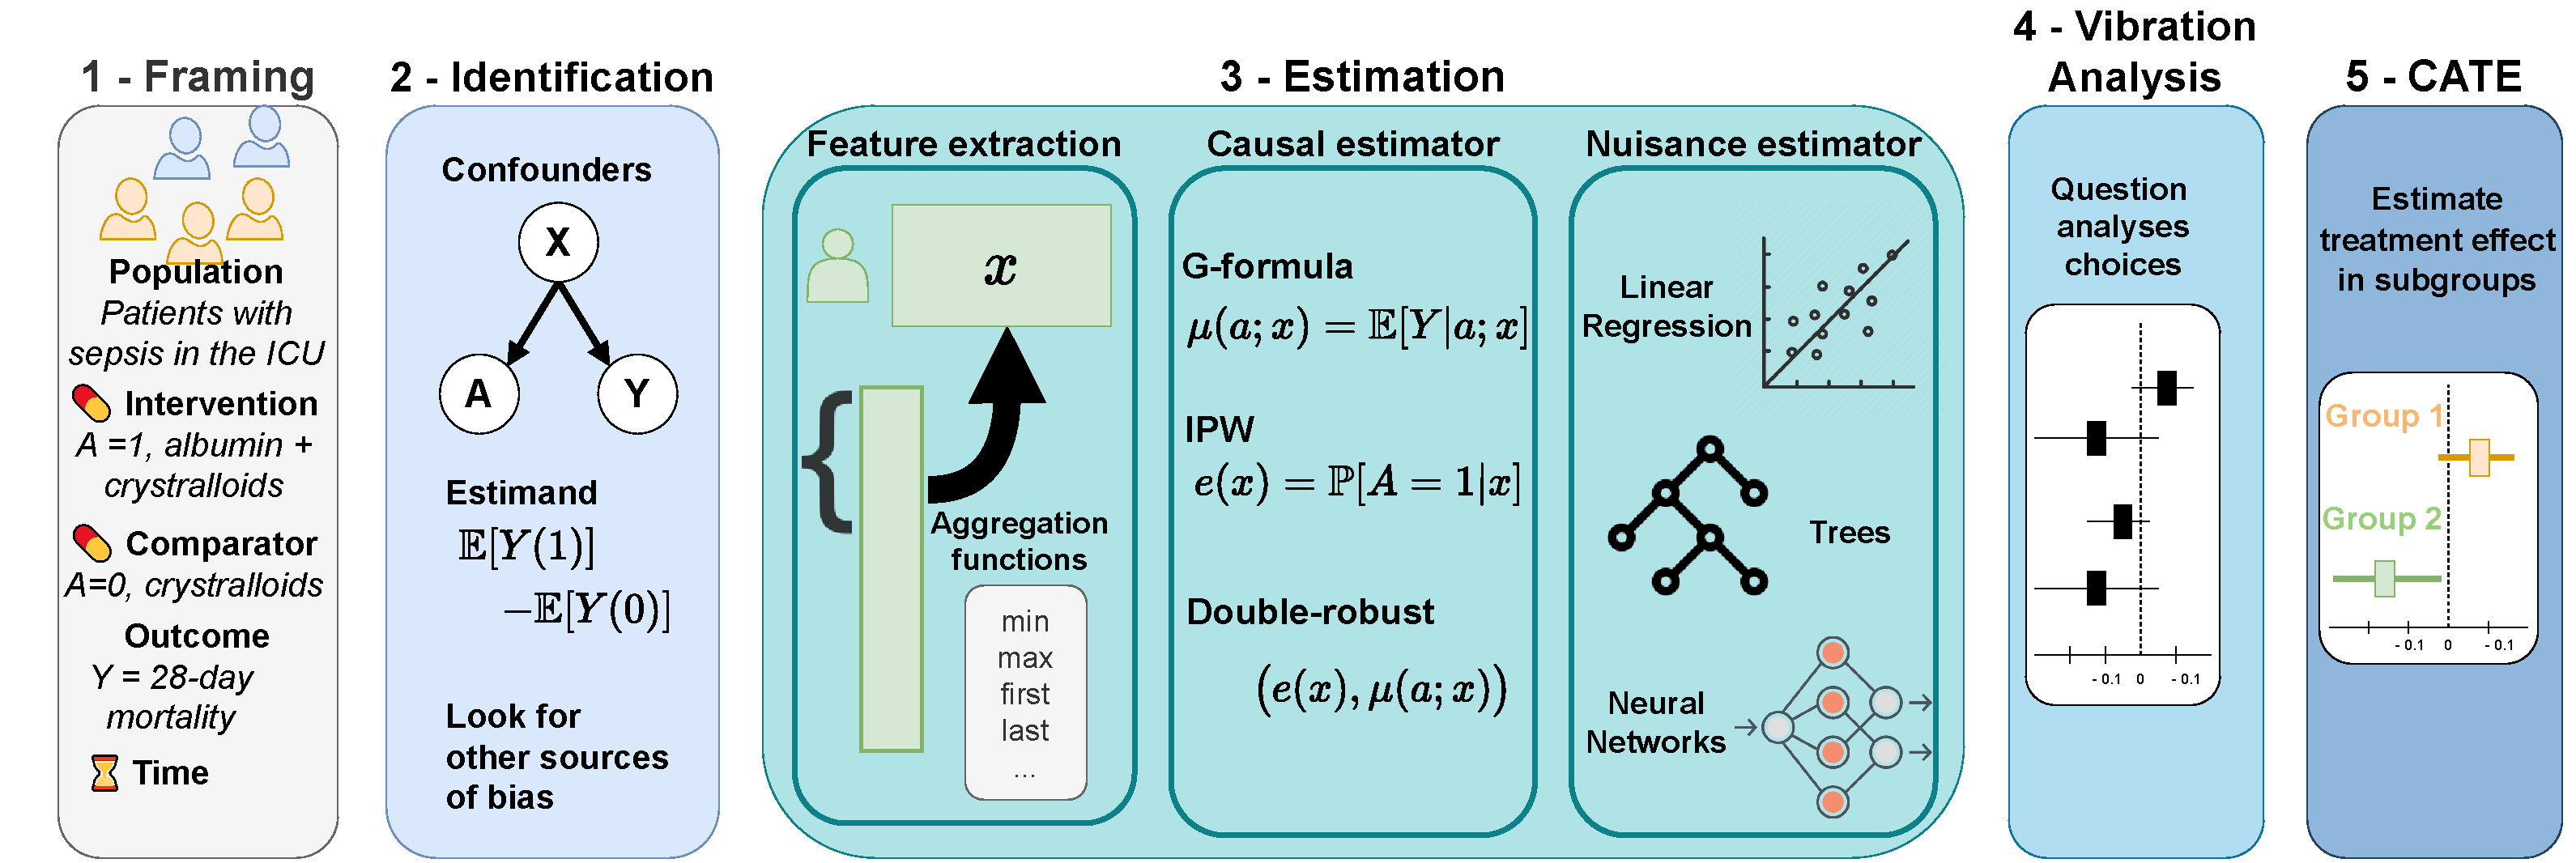
\includegraphics[width=0.9\linewidth]{img_final/Fig1.pdf}
  \caption{\textbf{Step-by-step analytic framework.}\\The complete
    inference pipeline confronts the analyst with
    many choices, some guided by domain knowledge, others
    by data insights. Making those choices explicit is necessary to ensure
    robustness and reproducibility.}\label{fig:inference_framework}
\end{figure*}



Whether or not using machine learning, many pitfalls threaten an analysis'
value for decision-making. To avoid these pitfalls, we outline a simple
step-by-step analytic framework illustrated in Fig
\ref{fig:inference_framework} for retrospective case-control studies. We frame
the medical question as a target trial \cite{hernan2021methods} to match the
design to an RCT giving the gold standard average effect. Then we probe for
heterogeneity --predictions on sub-groups--  going beyond what RCTs can
achieve.

\subsection*{Step 1: study design -- Frame the question to avoid biases}\label{sec:framing}


\begin{table*}[b!]
  \resizebox{\linewidth}{!}{%
    \begin{tabular}{|l|l|l|l|}
      \hline
      \multicolumn{1}{|c|}{\textbf{PICO component}} & \multicolumn{1}{c|}{\textbf{Description}}       & \multicolumn{1}{c|}{\textbf{Notation}}                 & \multicolumn{1}{c|}{\textbf{Example}}         \\ \hline
      \cellcolor{P}\textbf{Population}              & What is the target population of interest?      & $X \sim \mathbb{P}(X)$, the covariate distribution     & \makecell[l]{Patients with sepsis in the ICU} \\ \hline
      \cellcolor{I}\textbf{Intervention}            & What is the treatment?                          & \makecell[l]{$A \sim \mathbb{P}(A=1)=p_A$,                                                             \\ the probability to be treated} & Combination of crystalloids and albumin \\ \hline
      \cellcolor{C}\textbf{Control}                 & What is the clinically relevant comparator?     & $1-A \sim 1-p_A$                                       & Crystalloids only                             \\ \hline
      \cellcolor{O}\textbf{Outcome}                 & \makecell[l]{What are the outcomes to compare?} & \makecell[l]{$Y(1), Y(0) \sim \mathbb{P}(Y(1), Y(0))$,                                                 \\ the potential outcomes distribution}  & 28-day mortality \\ \hline
      \cellcolor{T}\textbf{Time}                    & \makecell[l]{Is the start of follow-up aligned                                                                                                           \\with intervention assignment?} & \makecell[l]{N/A}  & \makecell[l]{Intervention \\ within the first day} \\ \hline
    \end{tabular}%
  }\\
  \caption{{\bf PICO(T) components help to clearly define the
        medical question of interest.}}\label{table:picot}
\end{table*}


Grounding decisions on evidence needs well-framed questions, defined by their
PICO(T) components. Population, Intervention, Control, and Outcome
\cite{richardson1995well,riva2012your}, and in case of EHRs or claims data an
additional time component, are necessary to concord with a (hypothetical) target
randomized clinical trial \cite{hernan_using_2016,wang2023emulation} -- Table
\ref{table:picot}. A selection flowchart such as in
S5 Fig makes inclusion and exclusion choices for PICOT explicit.

Without care in defining these PICO(T) components, non-causal associations
between treatment and outcomes can easily be introduced into an analysis
\cite{catalogofbias}. The time-varying nature of EHR calls for checking
systematically of the Population and Time components by addressing two commonly
encountered types of bias.


\paragraph{Selection Bias:} In EHRs, outcomes and treatments are often not
directly available and need to be inferred from indirect events. These signals
could be missing not-at random, sometimes correlated with the treatment
allocation \cite{weiskopf2023healthcare}. For example, billing codes can be
strongly associated with case-severity and cost. Consider comparing the
effectiveness of fluid resuscitation with albumin to crystalloids. As albumin is
more costly, this treatment is more likely to have a sepsis billing code. On the
contrary, for patients treated with crystalloids, only the most severe cases
will have a billing code. Naively comparing patients would overestimate the
effect of albumin.

\paragraph{Immortal time bias:} Improper alignment of the inclusion defining
event and the intervention time is a major source of bias in time-varying data
\cite{suissa2008immortal,hernan2016specifying,wang2022understanding}. Immortal time bias (illustrated in S2 Fig) occurs when the follow-up period,
i.e. cohort entry, starts before the intervention, e.g. prescription for a
second-line treatment. In this case, the treated group will be biased towards
patients still alive at the time of assignment and thus overestimating the
effect size. Other frequent temporal biases are lead time bias
\cite{Oke2021leadtimebias,fu2021timing} or right censorship  \cite{hernan2016specifying}, and attrition bias
\cite{Bankhead2017attritionbias}. Good
practices include explicitly stating the cohort inclusion event   \cite[Chapter~10:Defining Cohorts]{ohdsi2019book} and defining
an appropriate grace period between starting time and the intervention
assignment \cite{hernan2016specifying}. At this step, a population timeline can
help.


\subsection*{Step 2: identification -- List necessary information to answer the causal question}\label{sec:identification}

The identification step builds a causal model to answer the research question.
%
Indeed, the analysis must compensate for differences between
treated and non-treated that are not due to the intervention
(\cite[chapter~1]{pearl2018book},
\cite[chapter~1]{hernan2020causal}).

\paragraph{Causal Assumptions}

Valid causal inference requires assumptions  \cite{rubin2005causal} --detailed
in S1 Appendix. The analyst should thus review the
plausibility of the following: 1) Unconfoundedness: after adjusting for the
confounders as ascertained by domain expert insight, treatment allocation should
be random; 2) Overlap --also called positivity-- the distribution of confounding
variables overlaps between the treated and controls --this is the only
assumption testable from data \cite{austin2015moving}--; 3) No interference
between units and consistency in the treatment, a reasonable assumption in most
clinical questions.

\paragraph{Categorizing covariates}
%
Potential predictors --covariates-- should be categorized depending on their
causal relations with the intervention and the outcome (illustrated in
S4 Fig): \emph{confounders} are common causes of the
intervention and the outcome; \emph{colliders} are caused by both the
intervention and the outcome; \emph{instrumental variables} are a cause of the
intervention but not the outcome, \emph{mediators} are caused by the
intervention and is a cause of the outcome. Finally, \emph{effect modifiers}
interact with the treatment, and thus
modulate the treatment effect in subpopulations \cite{attia2022proposal}.

To capture a valid causal effect, the analysis should only include confounders
and possible treatment-effect modifiers to study the resulting heterogeneity.
Regressing the outcome on instrumental and post-treatment variables (colliders
and mediators) will lead to biased causal estimates
\cite{vanderweele2019principles}. Drawing causal Directed Acyclic Graphs
(DAGs) \cite{greenland1999causal}, \emph{eg} with a webtool such as DAGitty \cite{textor2011dagitty}, helps capturing the relevant
variables and defining a suitable estimand or effect measure.

Unconfoundedness --inclusion of all confounders in the analysis-- is a strong
assumption that can be difficult to ascertain in practice applications. In these cases,
sensitivity analyses for omitted variable bias allow to test the robustness of
the results to missing confounders \cite{cinelli2020making}, proximal inference
can be used to leverage proxy of unobserved confounders
\cite{tchetgen2024introduction}, and the presence of a natural experiment or RCT might
identify the desired causal effect without unconfoundedness \cite[Chapter 5,
  9]{wager2020stats}.

The
\emph{estimand} is the final causal quantity estimated from the data.
Depending on the question, different estimands are better suited to contrast
the two potential outcomes E[Y(1)] and E[Y(0)] \cite{imbens_nonparametric_2004,colnet2023risk}. For continuous outcomes, risk
difference is a natural estimand, while for binary outcomes (e.g. events) the
choice of estimand depends on the scale. Whereas the risk difference is very
informative at the population level, e.g. for medico-economic decision-making,
the risk ratio and the hazard ratio are more informative at the level of
sub-groups or individuals \cite{colnet2023risk}.

\paragraph{Causal estimators}

A given estimand can be estimated through different methods. One can model the
outcome with regression models also known as
G-formula, \cite{robins1986role} and use it as a predictive counterfactual model
for all possible treatments for a given patient. Alternatively, one can model
the propensity of being treated for use in matching or Inverse Propensity
Weighting (IPW) \cite{austin2015moving}. Finally, doubly robust methods model
both the outcome and the treatment, benefiting from the convergence of both
models \cite{wager2020stats}. There is a variety of doubly robust models,
reviewed in S2 Appendix.

\subsection*{Step 3: Statistical estimation -- Compute the causal effect of interest}\label{sec:estimation}

%\paragraph{Confounder extraction}
%
%Measured variables extracted from the raw EHRs should match the confounders
%listed in the causal graph.

\paragraph{Confounder aggregation}
Confounders captured via measures collected over multiple time points must be
aggregated at the patient level. Simple forms of aggregation include taking the
first or last value before a time point, or an aggregate such as mean or median
over time. More elaborate choices may rely on hourly aggregations providing more
detailed information on the disease course such as vital signs. They may reduce
confounding bias between rapidly deteriorating and stable patients but also
increase the number of confounders making estimation more challenging
\cite{damour2020overlap}. The increase of variance occurs either in
arbitrarily small propensity scores for treatment models or in hazardous
extrapolation from one group to another for outcome model. If multiple
choices appear reasonable, one should compare them in a vibration analysis
(see \nameref{sec:vibration_analysis}).

Beyond tabular data, unstructured clinical text may capture confounding or
prognostic information \cite{horng2017creating,jiang2023health} which can be
added in the causal model \cite{zeng2022uncovering}.
However, high-dimensional
confounder space such as text may break the positivity assumption just as hourly
aggregation choices for measurements.

Missing covariate values might also be a source of confounding. Some statistical
estimators (such as forests) can directly incorporate them as supplementary
covariates. Others, such as linear models, require imputations.
S3 Appendix details general sanity checks for
imputation strategies when using statistical estimators.

\paragraph{Statistical estimation models of outcome and treatment}

The causal estimators use models of the outcome or the treatment --called
nuisances. There is currently no clear best practice to choose the corresponding
statistical model \cite{wendling2018comparing, dorie2019automated}. The
trade-off lies between simple models risking misspecification of the nuisance
parameters versus flexible models risking to overfit the data at small sample
sizes. Stacking models of different complexity as in a super-learner is a good
solution to navigate the trade-off \cite{van2007super,doutreligne2023select}.

\subsection*{Step 4: Vibration analysis -- Assess the robustness of the hypotheses}\label{sec:vibration_analysis}

Some choices in the pipeline may not be clear cut. Several options should then
be explored, to derive conceptual error bars going beyond a single statistical
model. When quantifying the bias from unobserved confounders, this process is
sometimes called sensitivity analysis \cite{schneeweiss2006sensitivity,thabane2013tutorial,fda_statistical_2021}.
Following \cite{patel2015assessment}, we use the term vibration analysis to
describe the sensitivity of the results to all analytic choices.

\subsection*{Step 5: Treatment heterogeneity -- Compute treatment effects on subpopulations}\label{sec:treatment_heterogeneity}

Once the causal design and corresponding estimators are established, they can be
used to explore the variation of treatment effects among subgroups. A
causally-grounded model can be used to predict the effect of the treatment from
all the covariates --confounders and effect modifiers-- the \emph{Conditional Average
  Treatment Effect} (CATE) \cite{robertson2021assessing}. Practically, CATEs can be estimated by regressing
an individual's predictions given by the causal estimator against the sources of
heterogeneity (details in S7 Appendix).


\section*{Application: evidence from MIMIC-IV on which resuscitation fluid to use}%
\label{sec:application_on_mimic_iv}

We now use the above framework to extract evidence-based decision rules for
resuscitation. Ensuring optimal organ perfusion in patients with septic shock
requires resuscitation by reestablishing circulatory volume with intravenous
fluids. While crystalloids are readily available, inexpensive and safe, a
large fraction of the administered volume is not retained in the vasculature.
Colloids offer the theoretical benefit of retaining more volume, but might be
more costly and have adverse effects \cite{annane2013effects}. Meta-analyses
from multiple pivotal RCTs found no effect of adding albumin to crystalloids
\cite{xu2014comparison,li2020resuscitation} on 28-day and 90-day mortality.  Given this
previous evidence, we thus expect no average effect of albumin on mortality in
sepsis patients. However, studies --RCT \cite{caironi2014albumin}  and observational
\cite{zhou2021early}-- have
found that septic-shock patients do benefit from albumin.

\paragraph{Emulated trial: Effect of albumin in combination with crystalloids
  compared to crystalloids alone on 28-day mortality in patients with sepsis}\label{emulated_trial}

Multiple published RCTs can validate the analysis pipeline before
investigating sub-population effects for individualized decisions. Using
MIMIC-IV \cite{johnson2020mimic}, we compare the magnitude of biases introduced by reasonable
choices in the different analytical steps recalled in Fig \ref{fig:study_summary}.

MIMIC-IV is a publicly available database that contains information from real
ICU stays of patients admitted to one tertiary academic medical center, Beth
Israel Deaconess Medical Center (BIDMC), in Boston, United States between 2008
and 2019. The data in MIMIC-IV has been previously de-identified, and the
institutional review boards of the Massachusetts Institute of Technology (No.
0403000206) and BIDMC (2001-P-001699/14) both approved the use of the database
for research. The database contains comprehensive information from ICU stays
including vital signs, laboratory measurements, medications, and mortality data
up to one year after discharge.

\begin{figure}[h!]
  \centering
  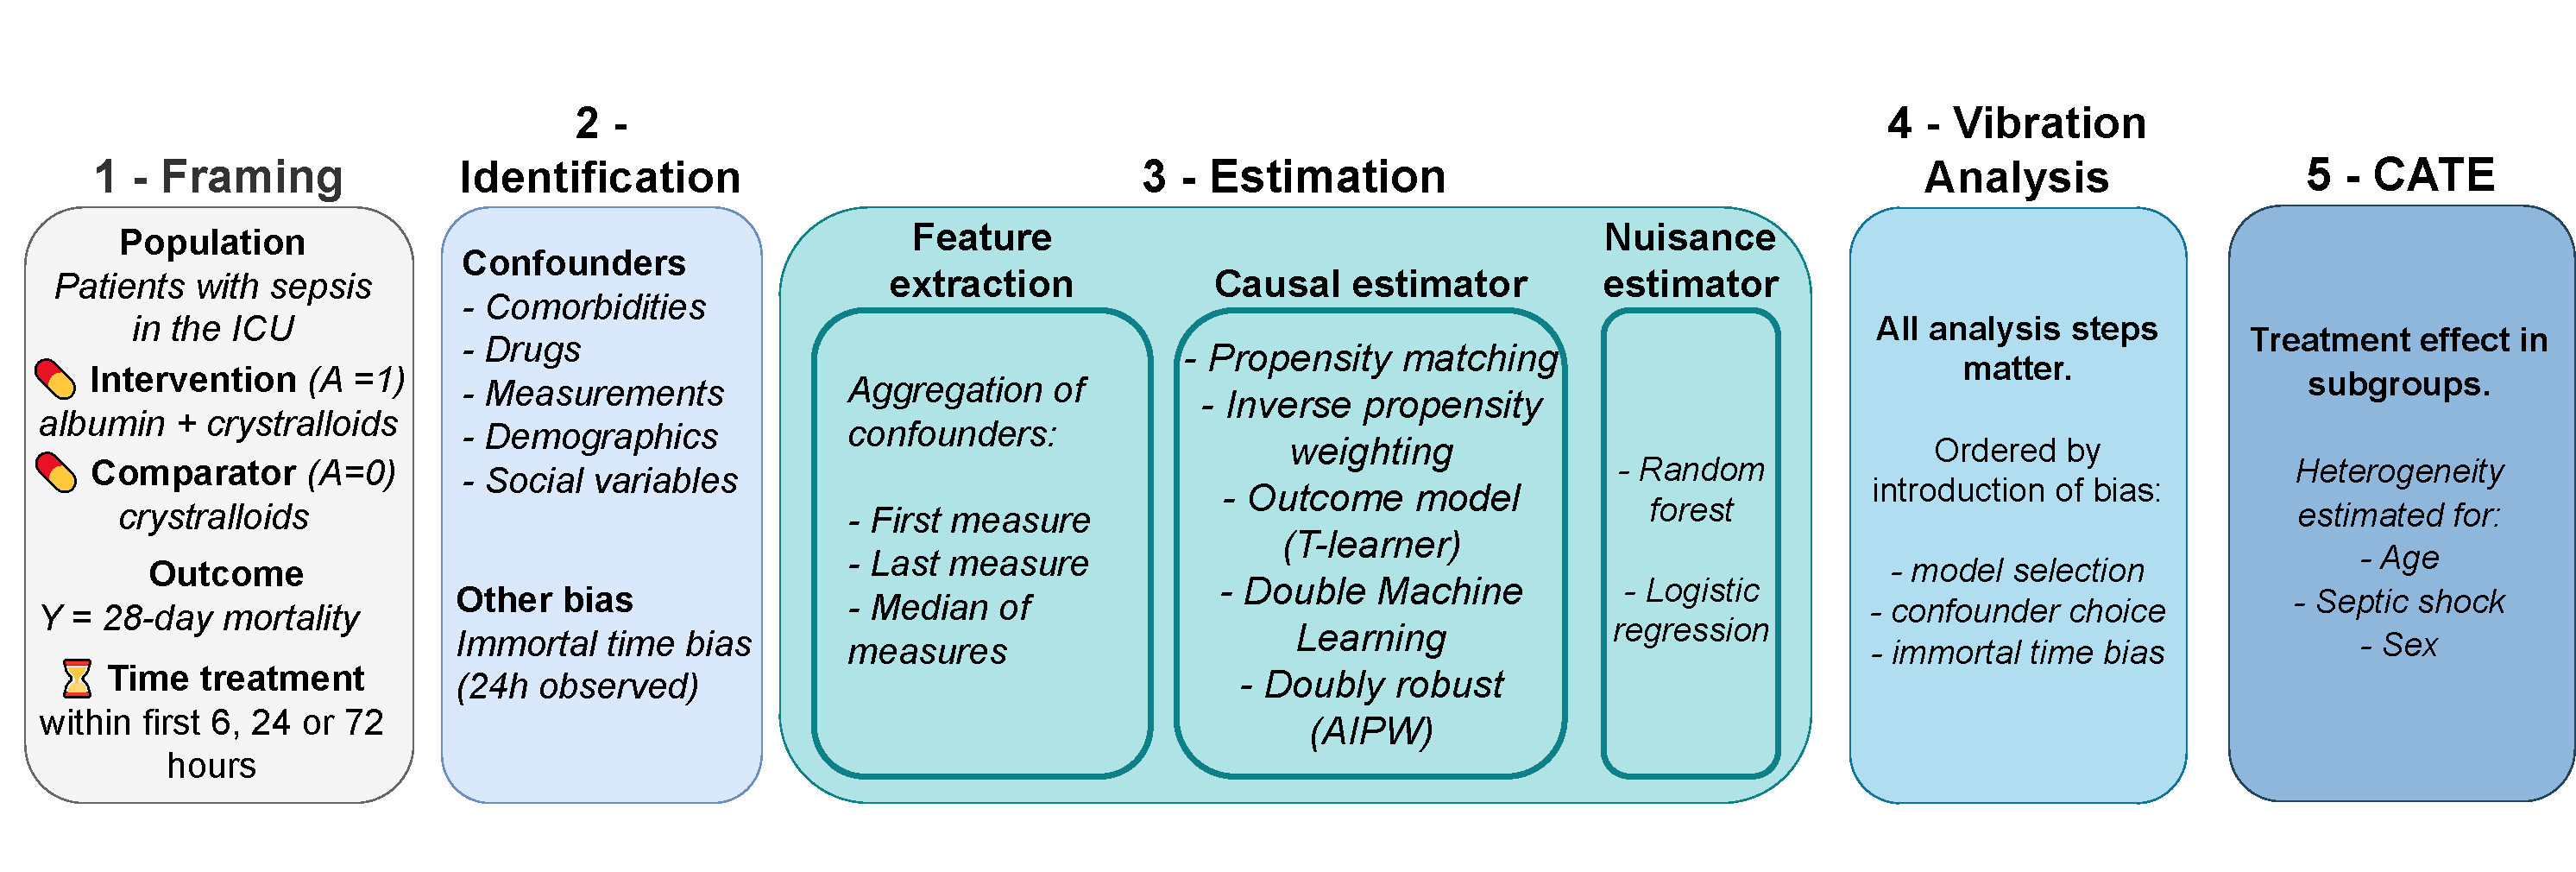
\includegraphics[width=\linewidth]{img_final/Fig2.pdf}
  \caption{\textbf{Application of the step-by-step framework on which resuscitation fluid to use.}}\label{fig:study_summary}
\end{figure}


\subsection*{Step 1: Study design -- effect of crystalloids on mortality in sepsis}%
\label{sec:framing_mimic_iv}

\begin{itemize}[leftmargin=2ex]
  \item \textcolor{P}{Population}: Patients with sepsis in an ICU stay according
        to the sepsis-3 definition. Other inclusion criteria: sufficient
        follow-up of at least 24 hours, and age over 18 years.
        S5 Fig details the selection flowchart and
        S1 Table the population
        characteristics.

  \item \textcolor{I}{Intervention}: Treatment with a combination of
        crystalloids and albumin during the first 24 hours of an ICU stay.

  \item \textcolor{C}{Control}: Treatment with crystalloids only in the first 24
        hours of an ICU stay.

  \item \textcolor{O}{Outcome}: 28-day mortality.

  \item \textcolor{T}{Time}: Follow-up begins after the first administration of
        crystalloids. Thus, we potentially introduce a small immortal time bias
        by allowing a time gap between follow-up and the start of the albumin
        treatment --see the full timeline in S3 Fig. Because
        we are only considering the first 24 hours of an ICU stay, we
        hypothesize that this gap is insufficient to affect our results. We test
        this hypothesis in the vibration analysis step.
\end{itemize}

In MIMIC-IV, these inclusion criteria yield 18,121 patients of which 3,559 were treated with a combination of crystalloids and albumin. While glycopeptide antibiotic therapy   was similar between both groups (51.8\% crystalloid vs 51.5\% crystalloids + albumin), aminoglycosides, carbapenems, and beta-lactams were more frequent in the crystalloid only group (2.0\% vs. 0.7\%, 4.3\% vs. 2.6\%, and 35.5\% vs. 13.8\%, respectively). The crystalloid only group was more frequently admitted as an emergency (57.3\% vs. 30.7\%). Vasopressors (80.2\% vs 41.7\%) and ventilation (96.8\% vs 87.0\%) were more prevalent in the treated populations, underlying the overall higher severity of patients receiving albumin (mean SOFA at admission 6.9 vs. 5.7).
Table \ref{table:albumin_for_sepsis:table1_simple} details
patient characteristics.


\begin{table}[h!]
  \centering\small
  \resizebox{\columnwidth}{!}{
    \begin{tabular}{llllll}
      \toprule
      {}                          & Missing & Overall      & Cristalloids only & Cristalloids + Albumin & P-Value \\
                                  &         &              &                   &                        &         \\
      \midrule
      n                           &         & 18421        & 14862             & 3559                   &         \\
      Female, n (\%)              &         & 7653 (41.5)  & 6322 (42.5)       & 1331 (37.4)            &         \\
      White, n (\%)               &         & 12366 (67.1) & 9808 (66.0)       & 2558 (71.9)            &         \\
      Emergency admission, n (\%) &         & 9605 (52.1)  & 8512 (57.3)       & 1093 (30.7)            &         \\
      admission\_age, mean (SD)   & 0       & 66.3 (16.2)  & 66.1 (16.8)       & 67.3 (13.1)            & <0.001  \\
      SOFA, mean (SD)             & 0       & 6.0 (3.5)    & 5.7 (3.4)         & 6.9 (3.6)              & <0.001  \\
      lactate, mean (SD)          & 4616    & 3.0 (2.5)    & 2.8 (2.4)         & 3.7 (2.6)              & <0.001  \\
      \bottomrule
    \end{tabular}

  }
  \\[.5ex]
  \caption{\textbf{Characteristics of the trial population measured on the first 24
      hours of ICU stay.}\\ S1 Table
    describes all confounders used in the analysis.}\label{table:albumin_for_sepsis:table1_simple}
\end{table}


\subsection*{Step 2: Identification -- listing confounders}\label{sec:identification_mimic_iv}

For confounders selection we use a causal DAG shown in Fig
S6 Fig. Gray confounders are not controlled for since
they are not available in the data. However, resulting confounding biases are
captured by proxies such as comorbidity scores (SOFA or SAPS II) or other
variables (eg. race, gender, age, weight).
%
S1 Table details confounders
summary statistics for treated and controls.


\paragraph{Causal estimators:}

We implemented multiple estimation strategies, including Inverse Propensity
Weighting (IPW), outcome modeling (G-formula) with T-Learner, Augmented Inverse
Propensity Weighting (AIPW) and Double Machine Learning (DML). We used the
python packages dowhy \cite{sharma2018tutorial} for IPW implementation and
EconML \cite{battocchi2019econml} for all other estimation strategies.
Confidence intervals were estimated by bootstrap (50 repetitions).
S2 Appendix and
S4 Appendix detail the estimators and the available Python
implementations. S3 Appendix details statistical considerations that we identified as important but missing in these packages, namely lack of cross fitting estimators, bad practices for imputation, or lack of closed form confidence intervals.

\subsection*{Step 3: Statistical estimation}\label{sec:estimation_mimic_iv}


\paragraph{Confounder aggregation:}

We tested multiple aggregations such as the last value before the start of the
follow-up period, the first observed value, and both the first and last values
as separated features. Missing values were median imputed for numerical
features, categorical variables were one-hot encoded (thus discarding missing values).


\paragraph{Outcome and treatment estimators:}

To model the outcome and treatment, we used two common but different
estimators: random forests and ridge logistic regression implemented with scikit-learn
\cite{pedregosa2011scikit}. We chose the
hyperparameters with a random search procedure (S5 Appendix). While logistic regression handles
predictors in a linear fashion, random forests bring the benefit of modeling
non-linear relations.


\subsection*{Step 4: Vibration analysis -- Comparing sources of systematic errors}%
\label{sec:vibration_analysis_mimic_iv}


\paragraph{Study design flaw -- Illustration of immortal time bias:}

To illustrate the risk of immortal-time bias, we vary the eligibility period of
treatment or control in a shorter or longer time window than 24 hours. As
explained in \nameref{sec:framing}, a longer eligibility period means that
patients are more likely to be treated if they survived up to the intervention
and hence the study is biased to overestimate the beneficial effect of the
intervention. Fig \ref{fig:vibration:itb} shows that longer eligibility
periods lead to albumin being markedly more efficient (detailed results with causal forest and other choices of aggregation in S8 Fig).

\begin{figure*}[h!]
  \begin{subfigure}[b]{\linewidth}
    \caption{\bfseries Framing -- Immortal Time Bias}\label{fig:vibration:itb}
    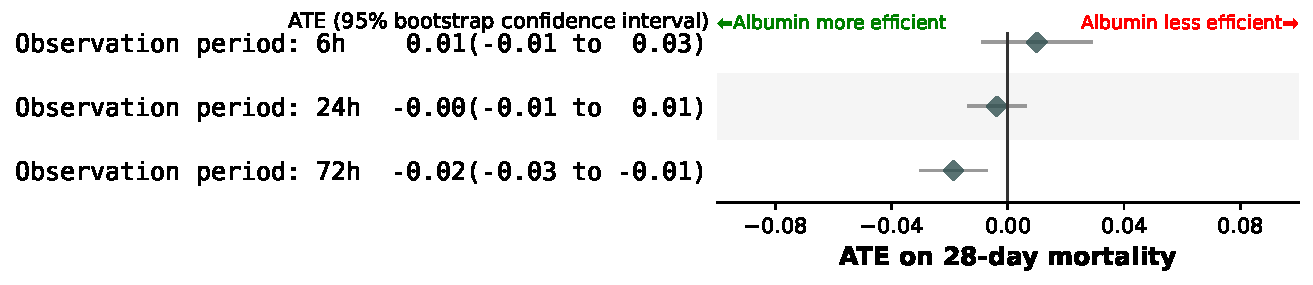
\includegraphics[width=0.765\linewidth, right]{img_final/Fig3a.pdf}
  \end{subfigure}
  \vfill
  \begin{subfigure}[b]{\linewidth}
    \centering
    \caption{\bfseries Identification -- confounders choice}\label{fig:vibration:confounders}
    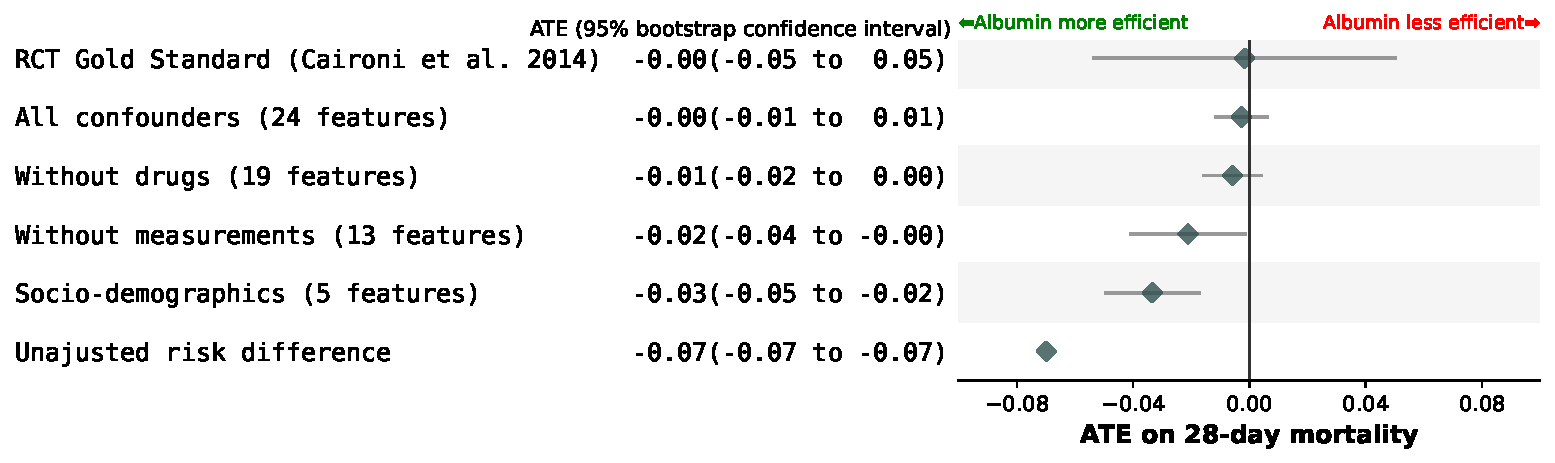
\includegraphics[width=.9\linewidth, right]{img_final/Fig3b.pdf}
  \end{subfigure}
  \vfill
  \begin{subfigure}[b]{\linewidth}
    \centering
    \caption{\bfseries Model selection}\label{fig:vibration:models}
    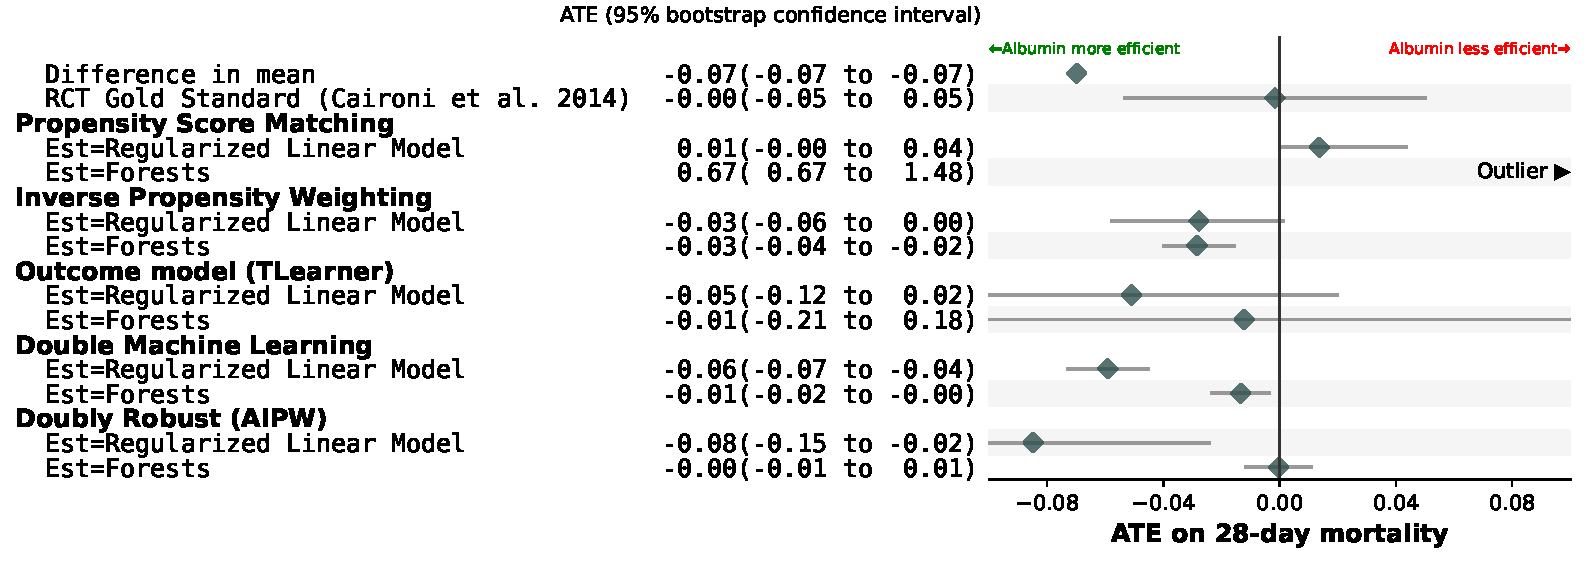
\includegraphics[width=0.891\linewidth, right]{img_final/Fig3c.pdf}
  \end{subfigure}
  \vfill
  \caption{\textbf{The effect of choices on the three
      analytical steps.}\\ All three
    analytical steps are equally important for the validity of the analysis.
    Fig \ref{fig:vibration:itb}) Framing step: Poor framing introduces time bias: A longer
    observation period (72h) artificially favors the efficacy of Albumin.
    Fig \ref{fig:vibration:confounders}) Identification step: Choosing less informed confounders set
    introduces increasing bias in the results. Fig \ref{fig:vibration:models}) Model selection step:
    Different estimators give different results. Score matching yields
    unconvincingly high estimates, inconsistent with the published RCT. With
    other causal approaches, using linear estimators for nuisances suggest a
    reduced mortality risk for albumin, while using forests for nuisance models
    points to no effect, which is consistent with the RCT gold standard.
    \\The diamonds depict the mean effect and the bar are the 95\% confidence
    intervals obtained respectively by 30, 30 and 50 bootstrap repetitions. For
    framing and identification, the estimator is a doubly robust learner (AIPW)
    with random forests for nuisances. Features are aggregated by taking the
    first and last measurements for all experiments.}\label{fig:vibration_analysis}
\end{figure*}


\paragraph{Confounder choice flaw} We consider other choice of confounding variables
(detailled in S6 Appendix). Fig
\ref{fig:vibration:confounders} shows that a less thorough choice, neglecting
the administrated drugs, makes little to no difference. Major errors, such as
omitting the biological measurements or using only socio-demographical
variables, lead to sizeable bias. This is consistent with the literature
highlighting the importance of a clinically valid DAG \cite{greenland1999causal}.

\paragraph{Estimation choices flaw -- Confounder aggregation, causal and nuisance estimators:}

Fig \ref{fig:vibration:models} shows varying confidence intervals (CI)
depending on the method. Doubly-robust methods provide the narrowest CIs,
whereas the outcome-regression methods have the largest CI. The estimates of the
forest models are closer to the consensus across prior studies (no effect) than
the logistic regression indicating a better fit of non-linear relationships. We
only report the first and last pre-treatment feature aggregation strategy, since
detailed analysis showed little differences for other aggregations (S7 Fig for complete results, and S9 Fig for a detailed study on aggregation choices). Both methodological studies \cite{naimi2023challenges} and
consistency with published RCTs suggest to prefer doubly-robust approaches.

\subsection*{Step 5: Treatment heterogeneity -- Which treatment for a sub-population?}%
\label{sec:treamtent_heterogeneity_mimic_iv}


With adequate choice of study design, confounding variables and causal
estimator, the average treatment effect matches well published findings:
Pooling evidence from high-quality RCTs, no effect of albumin in severe
sepsis was demonstrated for both 28-day mortality (odds ratio (OR) 0.93,
95\% CI 0.80-1.08) and 90-day mortality (OR 0.88, 95\% CI 0.761.01)
\cite{xu2014comparison}.
%
Having validated the analytical pipeline, we can use it to inform
decision-making. We explore
heterogeneity along four binary patient characteristics, displayed in Fig
\ref{fig:albumin_for_sepsis:cate_results}. We find that albumin is beneficial
with patient with septic shock consistent with one
RCT  \cite{caironi2014albumin}. It is also beneficial for older patients (age >=60) and males. S7 Appendix details the heterogeneity analysis.

\begin{figure}[h!]
  \begin{minipage}{.4\linewidth}
    \caption{\textbf{Subgroup distributions of Individual Treatment
        effects}:
      better treatment efficacy for patients older than 60 years, septic shock,
      and to a lower extent males. The final estimator is ridge regression. The
      boxes contain the $25^\text{th}$ and $75^\text{th}$ percentiles of the CATE
      distributions with the median indicated by the vertical line. The whiskers
      extend to 1.5 times the inter-quartile range of the
      distribution.}\label{fig:albumin_for_sepsis:cate_results}
  \end{minipage}%
  \hfill%
  \begin{minipage}{.6\linewidth}
    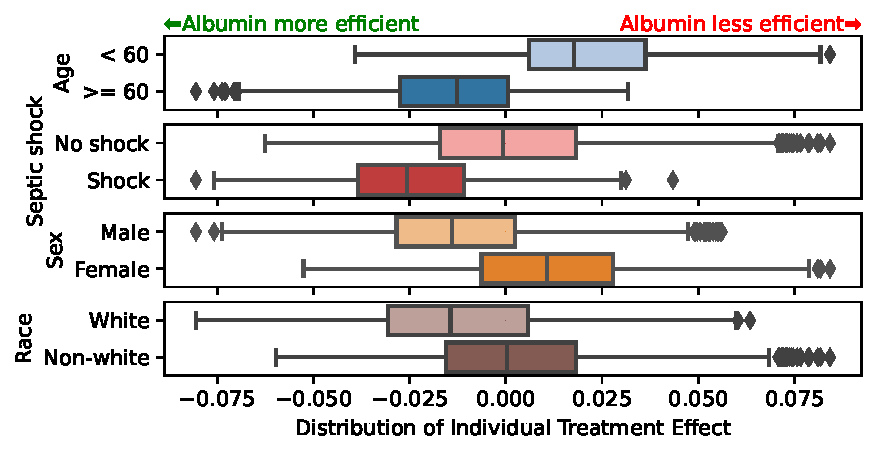
\includegraphics[width=\linewidth]{img_final/Fig4.pdf}
  \end{minipage}%
\end{figure}


\section*{Discussion and conclusion}\label{sec:discussion}

% -	Ideas of the discussion
% o	The three steps are important, list them in simple terms, but a sentence rather than a name
% o	We argue to anchor validity by comparing the average effect to a target trial, even when the goal of the analysis is heterogeneous effect. Importance of sub-population analysis to individualize decision
% o	No magic bullet
% o     Go back to decision-making
% o	Conclusion: racial bias and equity

Valid decision-making evidence from EHR data requires a clear causal framework.
Indeed, machine-learning algorithms have often extracted non-causal associations
between the intervention and the outcome, improper for decision-making
\cite{winkler2019association,badgeley2019deep,obermeyer2019dissecting}.
Machine learning studies in medicine often rely on an implicit causal
thinking, via a good understanding of the clinical settings.
A clear framework helps making
sure nothing falls through the cracks.

We have separated three steps important for causal validity: the choice
of study design, confounders, and estimators.
%
Regarding study design, major caveats arise from the time component,
where a poor choice of inclusion time easily brings in significant bias. Regarding choice of prediction
variables, forgetting some variables that explains both the treatment
allocation and the outcome leads to confounding bias, that however
remains small when these
variables capture weak links. Regarding choice of causal estimators,
preferring flexible models such as random forests reduces the bias, in
particular for doubly-robust estimators.
%
We have shown that all these three steps are equally important: paying no
attention to one of them leads to invalid estimates of treatment effect,
yet imperfect but plausible choices lead to small biases of the same
order of magnitude for all steps.
%
For instance, despite the emphasis often put on choice of confounders,
minor deviations from the expert's causal graph did not introduce
substantial bias (\ref{fig:vibration:confounders}), no larger than a too
rigid choice of estimator.
% Importance of reference target trial
To assert the validity of the analysis, we argue to relate as much as
possible the average effect to a reference target trial, even when the
goal is to capture the heterogeneity of the effect to individualize
decisions.
% Go back to decision-making
EHRs complement RCTs: RCTs cannot address all the
subpopulations and local practices
\cite{travers2007external,kennedy2015literature}. EHRs often cover many
individuals, with the diversity needed to model treatment
heterogeneity. The corresponding model can then inform better
decision-making \cite{prosperi2020causal}: a sub-population analysis  (as in Fig
\ref{fig:albumin_for_sepsis:cate_results}) can distill rules on which groups
of patients should receive a treatment. Beyond a sub-group perspective,
patient-specific estimates facilitate a personalized approach
to clinical decision-making \cite{kent2018personalized}.
% Focus on the medical question

Since the early 1980ies, researcher investigated the use of colloid fluids in
sepsis resuscitation due to their theoretical advantages. However, evidence has
long been conflicting. The debate was sparked anew when new synthetic colloid
solutions became available, but were later shown to have renal adverse effects
\cite{xu2014comparison}. As even large RCTs left unanswered questions,
researchers focused on meta-analyses. Here our analysis is in line with the
latest two meta-analyses \cite{xu2014comparison,li2020resuscitation}, as we
found no net benefit for resuscitation with albumin in septic patients overall,
but a possible slight benefit for patients with septic shock (see Fig.
\ref{fig:albumin_for_sepsis:cate_results}). While regular meta-analyses not
utilizing patient-level data are restricted in their sensitivity analyses, our
approach offers the benefit to investigate further potential effect modifiers
such as age, sex, or race.

% No magic bullet and its not all about ML
Even without considering a specific intervention, anchoring
machine-learning models on
causal mechanisms can make them more robust to distributional shift \cite{scholkopf2021toward},
thus safer and fairer for clinical use
\cite{richens2020improving,plecko2022causal}.
%
Yet it is important to keep in mind that better prediction is not per se
a goal in healthcare.
%
Establishing strong predictors might be less important than identifying
moderately strong but modifiable risk factors as established in the Framingham
cohort \cite{brand1976multivariate}, or optimizing population-wide cost-effectiveness instead of individual treatment effect.

No sophisticated data-processing tool can safeguard against
invalid study design or a major missing confounder, loopholes that can
undermine decision-making systems. Our framework helps the investigator
ensure
causal validity by outlining the important steps and relating average effects to
RCTs. Causal grounding of individual predictions should reduce the social
disparities that they reinforce
\cite{rajkomar2018ensuring,mitra2022future,ehrmann2023making}, as these are driven by
historical decisions and not biological mechanisms. At the population
level, it leads to better public health decisions. For instance, going
back to cardio-vascular diseases, the stakes are to go beyond risk
scores and also account for responder status when prescribing prevention
drugs.


\section*{Availability of data and materials}

The datasets are available on PhysioNet (
\url{https://doi.org/10.13026/6mm1-ek67}). We used MIMIC-IV.v2.2 The code for
data preprocessing and analyses are available on github
\url{https://github.com/soda-inria/causal_ehr_mimic/}.
The project was run on a laptop running Ubuntu 22.04.2 LTS with the following hardware: CPU 12th Gen Intel(R) Core(TM) i7-1270P with 16 threads and 15 GB of RAM.

% \section*{Fundings}
% This study was supported by an unrestricted educational grants to TS (Swiss
% National Science Foundation, P400PM\_194497 / 1) as well as an ERC grant to GV
% (Intercept-T2D HORIZON-HLTH-2022-STAYHLTH-02-01). LAC is funded by the National
% Institute of Health through NIBIB R01 EB017205.

\section*{Authors contributions}

MD and TS designed the study, MD performed the analysis and wrote the manuscript.
TS, JA, CM, LAC, GV reviewed and edited the manuscript.

\section*{Acknowledgments}

We thank all the PhysioNet team for their encouragements and support. In
particular: Fredrik Willumsen Haug, João Matos, Luis Nakayama, Sicheng Hao, Alistair Johnson.

\nolinenumbers

\begin{thebibliography}{100}

  \bibitem{rajkomar2018scalable}
  Rajkomar A, Oren E, Chen K, Dai AM, Hajaj N, Hardt M, et~al.
  \newblock Scalable and accurate deep learning with electronic health records.
  \newblock NPJ digital medicine. 2018;1(1):18.

  \bibitem{liu2019comparison}
  Liu X, Faes L, Kale AU, Wagner SK, Fu DJ, Bruynseels A, et~al.
  \newblock A comparison of deep learning performance against health-care professionals in detecting diseases from medical imaging: a systematic review and meta-analysis.
  \newblock The lancet digital health. 2019;1(6):e271--e297.

  \bibitem{li2020behrt}
  Li Y, Rao S, Solares JRA, Hassaine A, Ramakrishnan R, Canoy D, et~al.
  \newblock BEHRT: transformer for electronic health records.
  \newblock Scientific reports. 2020;10(1):1--12.

  \bibitem{beaulieu2021machine}
  Beaulieu-Jones BK, Yuan W, Brat GA, Beam AL, Weber G, Ruffin M, et~al.
  \newblock Machine learning for patient risk stratification: standing on, or looking over, the shoulders of clinicians?
  \newblock NPJ digital medicine. 2021;4(1):62.

  \bibitem{aggarwal2021diagnostic}
  Aggarwal R, Sounderajah V, Martin G, Ting DS, Karthikesalingam A, King D, et~al.
  \newblock Diagnostic accuracy of deep learning in medical imaging: a systematic review and meta-analysis.
  \newblock NPJ digital medicine. 2021;4(1):65.

  \bibitem{rajkomar2018ensuring}
  Rajkomar A, Hardt M, Howell MD, Corrado G, Chin MH.
  \newblock Ensuring fairness in machine learning to advance health equity.
  \newblock Annals of internal medicine. 2018;169(12):866--872.

  \bibitem{singh2022generalizability}
  Singh H, Mhasawade V, Chunara R.
  \newblock Generalizability challenges of mortality risk prediction models: A retrospective analysis on a multi-center database.
  \newblock PLOS Digital Health. 2022;1(4):e0000023.

  \bibitem{gichoya2022ai}
  Gichoya JW, Banerjee I, Bhimireddy AR, Burns JL, Celi LA, Chen LC, et~al.
  \newblock AI recognition of patient race in medical imaging: a modelling study.
  \newblock The Lancet Digital Health. 2022;4(6):e406--e414.

  \bibitem{seyyed2021underdiagnosis}
  Seyyed-Kalantari L, Zhang H, McDermott MB, Chen IY, Ghassemi M.
  \newblock Underdiagnosis bias of artificial intelligence algorithms applied to chest radiographs in under-served patient populations.
  \newblock Nature medicine. 2021;27(12):2176--2182.

  \bibitem{geirhos2020shortcut}
  Geirhos R, Jacobsen JH, Michaelis C, Zemel R, Brendel W, Bethge M, et~al.
  \newblock Shortcut learning in deep neural networks.
  \newblock Nature Machine Intelligence. 2020;2(11):665--673.

  \bibitem{winkler2019association}
  Winkler JK, Fink C, Toberer F, Enk A, Deinlein T, Hofmann-Wellenhof R, et~al.
  \newblock Association between surgical skin markings in dermoscopic images and diagnostic performance of a deep learning convolutional neural network for melanoma recognition.
  \newblock JAMA dermatology. 2019;155(10):1135--1141.

  \bibitem{degrave2021ai}
  DeGrave AJ, Janizek JD, Lee SI.
  \newblock AI for radiographic COVID-19 detection selects shortcuts over signal.
  \newblock Nature Machine Intelligence. 2021;3(7):610--619.

  \bibitem{badgeley2019deep}
  Badgeley MA, Zech JR, Oakden-Rayner L, Glicksberg BS, Liu M, Gale W, et~al.
  \newblock Deep learning predicts hip fracture using confounding patient and healthcare variables.
  \newblock NPJ digital medicine. 2019;2(1):31.

  \bibitem{obermeyer2019dissecting}
  Obermeyer Z, Powers B, Vogeli C, Mullainathan S.
  \newblock Dissecting racial bias in an algorithm used to manage the health of populations.
  \newblock Science. 2019;366(6464):447--453.

  \bibitem{yuan2021temporal}
  Yuan W, Beaulieu-Jones BK, Yu KH, Lipnick SL, Palmer N, Loscalzo J, et~al.
  \newblock Temporal bias in case-control design: preventing reliable predictions of the future.
  \newblock Nature communications. 2021;12(1):1107.

  \bibitem{wong2021external}
  Wong A, Otles E, Donnelly JP, Krumm A, McCullough J, DeTroyer-Cooley O, et~al.
  \newblock External validation of a widely implemented proprietary sepsis prediction model in hospitalized patients.
  \newblock JAMA Internal Medicine. 2021;181(8):1065--1070.

  \bibitem{prosperi2020causal}
  Prosperi M, Guo Y, Sperrin M, Koopman JS, Min JS, He X, et~al.
  \newblock Causal inference and counterfactual prediction in machine learning for actionable healthcare.
  \newblock Nature Machine Intelligence. 2020;2(7):369--375.

  \bibitem{plecko2022causal}
  Plecko D, Bareinboim E.
  \newblock Causal fairness analysis.
  \newblock arXiv preprint arXiv:220711385. 2022;.

  \bibitem{travers2007external}
  Travers J, Marsh S, Williams M, Weatherall M, Caldwell B, Shirtcliffe P, et~al.
  \newblock External validity of randomised controlled trials in asthma: to whom do the results of the trials apply?
  \newblock Thorax. 2007;62(3):219--223.

  \bibitem{averitt2020translating}
  Averitt AJ, Weng C, Ryan P, Perotte A.
  \newblock Translating evidence into practice: eligibility criteria fail to eliminate clinically significant differences between real-world and study populations.
  \newblock NPJ digital medicine. 2020;3(1):67.

  \bibitem{desai2021broadening}
  Desai RJ, Matheny ME, Johnson K, Marsolo K, Curtis LH, Nelson JC, et~al.
  \newblock Broadening the reach of the FDA Sentinel System: a roadmap for integrating electronic health record data in a causal analysis framework.
  \newblock NPJ digital medicine. 2021;4(1):170.

  \bibitem{rekkas2023standardized}
  Rekkas A, van Klaveren D, Ryan PB, Steyerberg EW, Kent DM, Rijnbeek PR.
  \newblock A standardized framework for risk-based assessment of treatment effect heterogeneity in observational healthcare databases.
  \newblock npj Digital Medicine. 2023;6(1):58.

  \bibitem{hernan2016specifying}
  Hernan MA, Sauer BC, Hernandez-Diaz S, Platt R, Shrier I.
  \newblock Specifying a target trial prevents immortal time bias and other self-inflicted injuries in observational analyses.
  \newblock Journal of clinical epidemiology. 2016;79:70--75.

  \bibitem{von2007strengthening}
  Von~Elm E, Altman DG, Egger M, Pocock SJ, G{\o}tzsche PC, Vandenbroucke JP.
  \newblock The Strengthening the Reporting of Observational Studies in Epidemiology (STROBE) statement: guidelines for reporting observational studies.
  \newblock The Lancet. 2007;370(9596):1453--1457.

  \bibitem{benchimol2015reporting}
  Benchimol EI, Smeeth L, Guttmann A, Harron K, Moher D, Petersen I, et~al.
  \newblock The REporting of studies Conducted using Observational Routinely-collected health Data (RECORD) statement.
  \newblock PLoS medicine. 2015;12(10):e1001885.

  \bibitem{hernan2020causal}
  Hernàn MA, Robins JM.
  \newblock Causal inference: What If.; 2020.

  \bibitem{schneeweiss2021conducting}
  Schneeweiss S, Patorno E.
  \newblock Conducting real-world evidence studies on the clinical outcomes of diabetes treatments.
  \newblock Endocrine Reviews. 2021;42(5):658--690.

  \bibitem{zeng2022uncovering}
  Zeng J, Gensheimer MF, Rubin DL, Athey S, Shachter RD.
  \newblock Uncovering interpretable potential confounders in electronic medical records.
  \newblock Nature Communications. 2022;13(1):1014.

  \bibitem{suissa2008immortal}
  Suissa S.
  \newblock Immortal time bias in pharmacoepidemiology.
  \newblock American journal of epidemiology. 2008;167(4):492--499.

  \bibitem{Oke2021leadtimebias}
  Oke J, Fanshawe T, Nunan D. Lead time bias, Catalogue of Bias Collaboration.; 2021.
  \newblock Available from: \url{https://catalogofbias.org/biases/lead-time-bias/}.

  \bibitem{fu2021timing}
  Fu EL, Evans M, Carrero JJ, Putter H, Clase CM, Caskey FJ, et~al.
  \newblock Timing of dialysis initiation to reduce mortality and cardiovascular events in advanced chronic kidney disease: nationwide cohort study.
  \newblock bmj. 2021;375.

  \bibitem{wang2022understanding}
  Wang SV, Sreedhara SK, Bessette LG, Schneeweiss S.
  \newblock Understanding variation in the results of real-world evidence studies that seem to address the same question.
  \newblock Journal of Clinical Epidemiology. 2022;151:161--170.

  \bibitem{Bankhead2017attritionbias}
  Bankhead~C ND Aronson~JK. Attrition bias, Catalogue of Bias Collaboration.; 2017.
  \newblock Available from: \url{https://catalogofbias.org/biases/attrition-bias/}.

  \bibitem{greenland1999causal}
  Greenland S, Pearl J, Robins JM.
  \newblock Causal diagrams for epidemiologic research.
  \newblock Epidemiology. 1999; p. 37--48.

  \bibitem{vanderweele2019principles}
  VanderWeele TJ.
  \newblock Principles of confounder selection.
  \newblock European journal of epidemiology. 2019;34:211--219.

  \bibitem{loh2021confounder}
  Loh WW, Vansteelandt S.
  \newblock Confounder selection strategies targeting stable treatment effect estimators.
  \newblock Statistics in Medicine. 2021;40(3):607--630.

  \bibitem{wang2023emulation}
  Wang SV, Schneeweiss S, Franklin JM, Desai RJ, Feldman W, Garry EM, et~al.
  \newblock Emulation of randomized clinical trials with nonrandomized database analyses: results of 32 clinical trials.
  \newblock JAMA. 2023;329(16):1376--1385.

  \bibitem{belloni2014high}
  Belloni A, Chernozhukov V, Hansen C.
  \newblock High-dimensional methods and inference on structural and treatment effects.
  \newblock Journal of Economic Perspectives. 2014;28(2):29--50.

  \bibitem{chernozhukov2018double}
  Chernozhukov V, Chetverikov D, Demirer M, Duflo E, Hansen C, Newey W, et~al.. Double/debiased machine learning for treatment and structural parameters; 2018.

  \bibitem{shalit2016tutorial}
  Shalit U, Sontag D. Causal Inference for Observational studies: Tutorial; 2016.
  \newblock Available from: \url{https://docplayer.net/64797211-Causal-inference-for-observational-studies.html}.

  \bibitem{sharma2018tutorial}
  Sharma A. Tutorial on causal inference and counterfactual reasoning; 2018.
  \newblock Available from: \url{https://causalinference.gitlab.io/kdd-tutorial/}.

  \bibitem{moraffah2021causal}
  Moraffah R, Sheth P, Karami M, Bhattacharya A, Wang Q, Tahir A, et~al.
  \newblock Causal inference for time series analysis: Problems, methods and evaluation.
  \newblock Knowledge and Information Systems. 2021;63:3041--3085.

  \bibitem{stuart2010matching}
  Stuart EA.
  \newblock Matching methods for causal inference: A review and a look forward.
  \newblock Statistical science: a review journal of the Institute of Mathematical Statistics. 2010;25(1):1.

  \bibitem{austin2015moving}
  Austin PC, Stuart EA.
  \newblock Moving towards best practice when using inverse probability of treatment weighting (IPTW) using the propensity score to estimate causal treatment effects in observational studies.
  \newblock Statistics in medicine. 2015;34(28):3661--3679.

  \bibitem{robins1986role}
  Robins JM, Greenland S.
  \newblock The role of model selection in causal inference from nonexperimental data.
  \newblock American Journal of Epidemiology. 1986;123(3):392--402.

  \bibitem{johansson2022generalization}
  Johansson FD, Shalit U, Kallus N, Sontag D.
  \newblock Generalization bounds and representation learning for estimation of potential outcomes and causal effects.
  \newblock The Journal of Machine Learning Research. 2022;23(1):7489--7538.

  \bibitem{schuler2017targeted}
  Schuler MS, Rose S.
  \newblock Targeted maximum likelihood estimation for causal inference in observational studies.
  \newblock American journal of epidemiology. 2017;185(1):65--73.

  \bibitem{dorie2019automated}
  Dorie V, Hill J, Shalit U, Scott M, Cervone D.
  \newblock Automated versus Do-It-Yourself Methods for Causal Inference.
  \newblock Statistical Science. 2019;34(1):43--68.

  \bibitem{alaa2019validating}
  Alaa A, Van Der~Schaar M.
  \newblock Validating causal inference models via influence functions.
  \newblock In: International Conference on Machine Learning. PMLR; 2019. p. 191--201.

  \bibitem{curth2021really}
  Curth A, Svensson D, Weatherall J, van~der Schaar M.
  \newblock Really doing great at estimating CATE? a critical look at ML benchmarking practices in treatment effect estimation.
  \newblock In: Thirty-fifth conference on neural information processing systems datasets and benchmarks track (round 2); 2021.

  \bibitem{johnson2020mimic}
  Johnson A, Bulgarelli L, Pollard T, Horng S, Celi LA, Mark R.
  \newblock Mimic-iv.
  \newblock PhysioNet Available online at: https://physionet org/content/mimiciv/10/(accessed August 23, 2021). 2020;.

  \bibitem{hernan2021methods}
  Hernan MA.
  \newblock Methods of public health research--strengthening causal inference from observational data.
  \newblock New England Journal of Medicine. 2021;385(15):1345--1348.

  \bibitem{richardson1995well}
  Richardson WS, Wilson MC, Nishikawa J, Hayward RS, et~al.
  \newblock The well-built clinical question: a key to evidence-based decisions.
  \newblock Acp j club. 1995;123(3):A12--A13.

  \bibitem{riva2012your}
  Riva JJ, Malik KM, Burnie SJ, Endicott AR, Busse JW.
  \newblock What is your research question? An introduction to the PICOT format for clinicians.
  \newblock The Journal of the Canadian Chiropractic Association. 2012;56(3):167.

  \bibitem{hernan_using_2016}
  Hernán MA, Robins JM.
  \newblock Using {Big} {Data} to {Emulate} a {Target} {Trial} {When} a {Randomized} {Trial} {Is} {Not} {Available}.
  \newblock American Journal of Epidemiology. 2016;183(8).

  \bibitem{catalogofbias}
  Catalogue of Bias Collaboration; 2023.
  \newblock Available from: \url{https://catalogofbias.org/biases/}.

  \bibitem{weiskopf2023healthcare}
  Weiskopf NG, Dorr DA, Jackson C, Lehmann HP, Thompson CA.
  \newblock Healthcare utilization is a collider: an introduction to collider bias in EHR data reuse.
  \newblock Journal of the American Medical Informatics Association. 2023; p. ocad013.

  \bibitem{ohdsi2019book}
  OHDSI.
  \newblock The Book of OHDSI: Observational Health Data Sciences and Informatics.
  \newblock OHDSI; 2021.
  \newblock Available from: \url{https://ohdsi.github.io/TheBookOfOhdsi/}.

  \bibitem{pearl2018book}
  Pearl J, Mackenzie D.
  \newblock The book of why: the new science of cause and effect.
  \newblock Basic books; 2018.

  \bibitem{rubin2005causal}
  Rubin DB.
  \newblock Causal inference using potential outcomes: Design, modeling, decisions.
  \newblock Journal of the American Statistical Association. 2005;100(469):322--331.

  \bibitem{attia2022proposal}
  Attia J, Holliday E, Oldmeadow C. A proposal for capturing interaction and effect modification using DAGs; 2022.

  \bibitem{textor2011dagitty}
  Textor J, Hardt J, Kn{\"u}ppel S.
  \newblock DAGitty: a graphical tool for analyzing causal diagrams.
  \newblock Epidemiology. 2011;22(5):745.

  \bibitem{cinelli2020making}
  Cinelli C, Hazlett C.
  \newblock Making sense of sensitivity: Extending omitted variable bias.
  \newblock Journal of the Royal Statistical Society Series B: Statistical Methodology. 2020;82(1):39--67.

  \bibitem{tchetgen2024introduction}
  Tchetgen~Tchetgen EJ, Ying A, Cui Y, Shi X, Miao W.
  \newblock An introduction to proximal causal inference.
  \newblock Statistical Science. 2024;39(3):375--390.

  \bibitem{wager2020stats}
  Wager S. Stats 361: Causal inference; 2020.

  \bibitem{imbens_nonparametric_2004}
  Imbens GW.
  \newblock Nonparametric {Estimation} of {Average} {Treatment} {Effects} {Under} {Exogeneity}: {A} {Review}.
  \newblock The Review of Economics and Statistics. 2004;86(1):4--29.

  \bibitem{colnet2023risk}
  Colnet B, Josse J, Varoquaux G, Scornet E.
  \newblock Risk ratio, odds ratio, risk difference... Which causal measure is easier to generalize?
  \newblock arXiv preprint arXiv:230316008. 2023;.

  \bibitem{damour2020overlap}
  D'Amour A, Ding P, Feller A, Lei L, Sekhon J.
  \newblock Overlap in observational studies with high-dimensional covariates.
  \newblock Journal of Econometrics. 2021;221(2):644--654.

  \bibitem{horng2017creating}
  Horng S, Sontag DA, Halpern Y, Jernite Y, Shapiro NI, Nathanson LA.
  \newblock Creating an automated trigger for sepsis clinical decision support at emergency department triage using machine learning.
  \newblock PloS one. 2017;12(4):e0174708.

  \bibitem{jiang2023health}
  Jiang LY, Liu XC, Nejatian NP, Nasir-Moin M, Wang D, Abidin A, et~al.
  \newblock Health system-scale language models are all-purpose prediction engines.
  \newblock Nature. 2023; p. 1--6.

  \bibitem{wendling2018comparing}
  Wendling T, Jung K, Callahan A, Schuler A, Shah NH, Gallego B.
  \newblock Comparing methods for estimation of heterogeneous treatment effects using observational data from health care databases.
  \newblock Statistics in medicine. 2018;37(23):3309--3324.

  \bibitem{van2007super}
  Van~der Laan MJ, Polley EC, Hubbard AE.
  \newblock Super learner.
  \newblock Statistical applications in genetics and molecular biology. 2007;6(1).

  \bibitem{doutreligne2023select}
  Doutreligne M, Varoquaux G.
  \newblock How to select predictive models for causal inference?
  \newblock arXiv preprint arXiv:230200370. 2023;.

  \bibitem{schneeweiss2006sensitivity}
  Schneeweiss S.
  \newblock Sensitivity analysis and external adjustment for unmeasured confounders in epidemiologic database studies of therapeutics.
  \newblock Pharmacoepidemiology and drug safety. 2006;15(5):291--303.

  \bibitem{thabane2013tutorial}
  Thabane L, Mbuagbaw L, Zhang S, Samaan Z, Marcucci M, Ye C, et~al.
  \newblock A tutorial on sensitivity analyses in clinical trials: the what, why, when and how.
  \newblock BMC medical research methodology. 2013;13(1):1--12.

  \bibitem{fda_statistical_2021}
  FDA.
  \newblock Statistical Principles for Clinical Trials: Addendum: Estimands and Sensitivity Analysis in Clinical Trials.
  \newblock FDA; 2021.

  \bibitem{patel2015assessment}
  Patel CJ, Burford B, Ioannidis JP.
  \newblock Assessment of vibration of effects due to model specification can demonstrate the instability of observational associations.
  \newblock Journal of clinical epidemiology. 2015;68(9):1046--1058.

  \bibitem{robertson2021assessing}
  Robertson SE, Leith A, Schmid CH, Dahabreh IJ.
  \newblock Assessing heterogeneity of treatment effects in observational studies.
  \newblock American Journal of Epidemiology. 2021;190(6):1088--1100.

  \bibitem{annane2013effects}
  Annane D, Siami S, Jaber S, Martin C, Elatrous S, Declere AD, et~al.
  \newblock Effects of fluid resuscitation with colloids vs crystalloids on mortality in critically ill patients presenting with hypovolemic shock: the CRISTAL randomized trial.
  \newblock Jama. 2013;310(17):1809--1817.

  \bibitem{xu2014comparison}
  Xu JY, Chen QH, Xie JF, Pan C, Liu SQ, Huang LW, et~al.
  \newblock Comparison of the effects of albumin and crystalloid on mortality in adult patients with severe sepsis and septic shock: a meta-analysis of randomized clinical trials.
  \newblock Critical Care. 2014;18(6):1--8.

  \bibitem{li2020resuscitation}
  Li B, Zhao H, Zhang J, Yan Q, Li T, Liu L.
  \newblock Resuscitation fluids in septic shock: a network meta-analysis of randomized controlled trials.
  \newblock Shock. 2020;53(6):679--685.

  \bibitem{caironi2014albumin}
  Caironi P, Tognoni G, Masson S, Fumagalli R, Pesenti A, Romero M, et~al.
  \newblock Albumin replacement in patients with severe sepsis or septic shock.
  \newblock New England Journal of Medicine. 2014;370(15):1412--1421.

  \bibitem{zhou2021early}
  Zhou S, Zeng Z, Wei H, Sha T, An S.
  \newblock Early combination of albumin with crystalloids administration might be beneficial for the survival of septic patients: a retrospective analysis from MIMIC-IV database.
  \newblock Annals of intensive care. 2021;11:1--10.

  \bibitem{battocchi2019econml}
  Battocchi K, Dillon E, Hei M, Lewis G, Oka P, Oprescu M, et~al.. {EconML}: {A Python Package for ML-Based Heterogeneous Treatment Effects Estimation}; 2019.
  \newblock Available from: \url{https://github.com/py-why/EconML}.

  \bibitem{pedregosa2011scikit}
  Pedregosa F, Varoquaux G, Gramfort A, Michel V, Thirion B, Grisel O, et~al.
  \newblock Scikit-learn: Machine learning in Python.
  \newblock the Journal of machine Learning research. 2011;12:2825--2830.

  \bibitem{naimi2023challenges}
  Naimi AI, Mishler AE, Kennedy EH.
  \newblock Challenges in obtaining valid causal effect estimates with machine learning algorithms.
  \newblock American Journal of Epidemiology. 2023;192(9):1536--1544.

  \bibitem{kennedy2015literature}
  Kennedy-Martin T, Curtis S, Faries D, Robinson S, Johnston J.
  \newblock A literature review on the representativeness of randomized controlled trial samples and implications for the external validity of trial results.
  \newblock Trials. 2015;16:1--14.

  \bibitem{kent2018personalized}
  Kent DM, Steyerberg E, van Klaveren D.
  \newblock Personalized evidence based medicine: predictive approaches to heterogeneous treatment effects.
  \newblock Bmj. 2018;363.

  \bibitem{scholkopf2021toward}
  Schölkopf B, Locatello F, Bauer S, Ke NR, Kalchbrenner N, Goyal A, et~al.
  \newblock Toward causal representation learning.
  \newblock Proceedings of the IEEE. 2021;109(5):612--634.

  \bibitem{richens2020improving}
  Richens JG, Lee CM, Johri S.
  \newblock Improving the accuracy of medical diagnosis with causal machine learning.
  \newblock Nature communications. 2020;11(1):3923.

  \bibitem{brand1976multivariate}
  Brand RJ, Rosenman RH, Sholtz RI, Friedman M.
  \newblock Multivariate prediction of coronary heart disease in the Western Collaborative Group Study compared to the findings of the Framingham study.
  \newblock Circulation. 1976;53(2):348--355.

  \bibitem{mitra2022future}
  Mitra N, Roy J, Small D.
  \newblock The Future of Causal Inference.
  \newblock American Journal of Epidemiology. 2022;191(10):1671--1676.

  \bibitem{ehrmann2023making}
  Ehrmann DE, Joshi S, Goodfellow SD, Mazwi ML, Eytan D.
  \newblock Making machine learning matter to clinicians: model actionability in medical decision-making.
  \newblock NPJ Digital Medicine. 2023;6(1):7.

  \bibitem{score22021score2}
  working group S.
  \newblock SCORE2 risk prediction algorithms: new models to estimate 10-year risk of cardiovascular disease in Europe.
  \newblock European heart journal. 2021;42(25):2439--2454.

  \bibitem{bretthauer2013principles}
  Bretthauer M, Kalager M.
  \newblock Principles, effectiveness and caveats in screening for cancer.
  \newblock Journal of British Surgery. 2013;100(1):55--65.

  \bibitem{lee2020immortaltimebias}
  Lee H, Nunan D. Immortal time bias, Catalogue of Bias Collaboration.; 2020.
  \newblock Available from: \url{https://catalogofbias.org/biases/immortaltimebias/}.

  \bibitem{rosenbaum1983central}
  Rosenbaum PR, Rubin DB.
  \newblock The central role of the propensity score in observational studies for causal effects.
  \newblock Biometrika;70:41--55.

  \bibitem{chernozhukov2022long}
  Chernozhukov V, Cinelli C, Newey W, Sharma A, Syrgkanis V.
  \newblock Long story short: Omitted variable bias in causal machine learning.
  \newblock National Bureau of Economic Research; 2022.

  \bibitem{jesson2020identifying}
  Jesson A, Mindermann S, Shalit U, Gal Y.
  \newblock Identifying causal-effect inference failure with uncertainty-aware models.
  \newblock Advances in Neural Information Processing Systems. 2020;33:11637--11649.

  \bibitem{snowden2011implementation}
  Snowden JM, Rose S, Mortimer KM.
  \newblock Implementation of G-computation on a simulated data set: demonstration of a causal inference technique.
  \newblock American journal of epidemiology. 2011;173(7):731--738.

  \bibitem{abadie2008failure}
  Abadie A, Imbens GW.
  \newblock On the failure of the bootstrap for matching estimators.
  \newblock Econometrica. 2008;76(6):1537--1557.

  \bibitem{robins1994estimation}
  Robins JM, Rotnitzky A, Zhao LP.
  \newblock Estimation of regression coefficients when some regressors are not always observed.
  \newblock Journal of the American statistical Association. 1994;89(427):846--866.

  \bibitem{foster2019orthogonal}
  Foster DJ, Syrgkanis V.
  \newblock Orthogonal statistical learning.
  \newblock arXiv preprint arXiv:190109036. 2019;.

  \bibitem{nie2021quasi}
  Nie X, Wager S.
  \newblock Quasi-oracle estimation of heterogeneous treatment effects.
  \newblock Biometrika. 2021;108(2):299--319.

  \bibitem{robinson1988root}
  Robinson PM.
  \newblock Root-N-consistent semiparametric regression.
  \newblock Econometrica: Journal of the Econometric Society. 1988; p. 931--954.

  \bibitem{sharma2020dowhy}
  Sharma A, Kiciman E.
  \newblock DoWhy: An end-to-end library for causal inference.
  \newblock arXiv preprint arXiv:201104216. 2020;.

  \bibitem{bouthillier2021accounting}
  Bouthillier X, Delaunay P, Bronzi M, Trofimov A, Nichyporuk B, Szeto J, et~al.
  \newblock Accounting for variance in machine learning benchmarks.
  \newblock Proceedings of Machine Learning and Systems. 2021;3:747--769.

  \bibitem{safe2007saline}
  Investigators SS.
  \newblock Saline or albumin for fluid resuscitation in patients with traumatic brain injury.
  \newblock New England Journal of Medicine. 2007;357(9):874--884.

\end{thebibliography}


\clearpage

\section*{Supporting information}

\paragraph*{S1 Fig.}
\label{apd:motivating_example}
{\bf Motivating example: Failure of predictive models to predict mortality
  from pretreatment variables.}

\paragraph*{S2 Fig.}
\label{apd:immortal_time_bias}
{\bf Immortal time bias illustration.}

\paragraph*{S3 Fig.}
\label{apd:graphical_timeline}
{\bf Graphical timeline.}

\paragraph*{S4 Fig.}
\label{apd:causal_variables}
{\bf Types of causal variables.}

\paragraph*{S5 Fig}
\label{apd:selection_flowchart}
{\bf Selection flowchart.}

\paragraph*{S6 Fig}
\label{apd:causal_diagram_albumin}
{\bf Directed Acyclic Graph.}

\paragraph*{S7 Fig}
\label{apd:detailed_results}
{\bf Complete results for the main analysis.}

\paragraph*{S8 Fig}
\label{apd:detailed_results_itb}
{\bf Complete results for the Immortal time bias.}

\paragraph*{S9 Fig}
\label{apd:vibration_analysis_for_aggregation}
{\bf Vibration analysis for aggregation.}

\paragraph*{S1 Appendix}
\label{apd:causal_assumptions}
{\bf Assumptions: what is needed for causal inference from observational studies.}

\paragraph*{S2 Appendix}
\label{apd:causal_estimators}
{\bf Major causal-inference methods: When to use which estimator?}

\paragraph*{S3 Appendix}
\label{apd:statistical_considerations}
{\bf Statistical considerations when implementing
  estimation.}

\paragraph*{S4 Appendix}
\label{apd:packages}
{\bf Packages for causal estimation in the python ecosystem.}

\paragraph*{S5 Appendix}
\label{apd:hyper_parameter_search}
{\bf Hyper-parameter search for the nuisance models.}

\paragraph*{S6 Appendix}
\label{apd:vibration_analysis_for_confounders}
{\bf Deviating from expert ignorability -- Impact of smaller confounders sets.}

\paragraph*{S7 Appendix}
\label{apd:hte}
{\bf Details on treatment heterogeneity analysis.}

\paragraph*{S1 Table}
\label{apd:albumin_for_sepsis:table1_complete}
{\bf Complete description of the confounders for the main analysis.}

\end{document}

